\documentclass{beamer}
\usepackage{tikz}
\usepackage{algorithm}
\usepackage[algo2e]{algorithm2e}
\usepackage[noend]{algpseudocode}
\usecolortheme{orchid}
\usepackage{slashbox}
\usepackage{ragged2e}


\mode<beamer>{\setbeamertemplate{blocks}[rounded][shadow=true]}

%\setbeamercolor{block example}{fg=blue, bg=black!20}
\setbeamertemplate{bibliography item}[text]


\title{Evaluation of Spell Correction on Noisy OCR Data }

\author[shortname]{Aayushee Gupta \inst{1} \\{\tiny aayushee1230@iiitd.ac.in} \and \\Haimonti Dutta \inst{2} \\{\tiny haimonti@buffalo.edu}}
\institute[shortinst]{\inst{1} Department of Computer Science, Indraprastha Institute of Information Technology, Delhi \and %
                     \inst{2} Department of Management Science and Systems, School of Management, University at Buffalo, New York}


%\author[shortname]{Aayushee Gupta \\{\tiny aayushee1230@iiitd.ac.in}  \\Indraprastha Institute of Information Technology, Delhi  %\and  \\Haimonti Dutta \\{\tiny haimonti@buffalo.edu} \\School of Management University, Buffalo}


%\author{Haimonti Dutta\\{\tiny haimonti@buffalo.edu}}
%\institute{School of Management University, Buffalo}
\date{October 31, 2015}
\begin{document}
\maketitle


\AtBeginSection[]
{
\begin{frame}{Agenda}
\tableofcontents[currentsection]
\end{frame}
}
%hideothersubsections
%MOTIVATION
\section{Motivation}

\begin{frame}
\frametitle{Motivation}
\begin{itemize}
\item 
Optical Character Recognition (OCR) is the electronic translation of handwritten, typewritten or printed text into machine translated images
\item
It has wide applications in the fields of banking, healthcare, digital libraries, handwriting recognition,etc.\cite{singh2012survey}
\end{itemize}
\begin{figure}[ht]
%\begin{center}
\includegraphics[scale=0.35]{images/handwriting.jpg}
\hspace{0.2in}
\includegraphics[scale=0.15]{images/printedOCR.jpg}
%\end{center}
\end{figure}

\end{frame}

\begin{frame}
\frametitle{An example from digital humanities}
\begin{figure}[ht]
\begin{center}
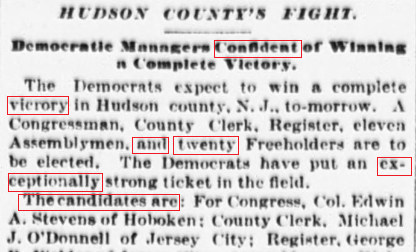
\includegraphics[scale=0.5]{images/originalimage}
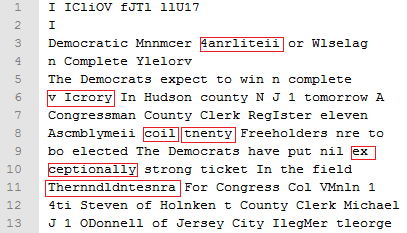
\includegraphics[scale=0.5]{images/ocr}
\caption{Scanned newspaper image and its corresponding noisy OCR text}
\end{center}
\end{figure}
\end{frame}

\begin{frame}
\frametitle{Motivation}
\begin{itemize}
 \justifying
\item
Spell correction becomes essential as the OCR process generates a lot of noisy text
\item Many algorithms exist in literature for automatic spell correction.
\item \textcolor{red}{\textbf{But how good are they?}}
\item A major problem that surfaces when evaluating the spell correction process is that the text has to be verified against the original text (ground truth) to estimate its performance. 
 \begin{itemize}
 \item Requires alignment of three parallel corpora - noisy OCR text, text corrected by software, ground truth (often manually verified)
 \end{itemize}
%\item This one-to-one verification may lead to word alignment problems, since the corrected and original text can be of different lengths.
\end{itemize}
\end{frame}

\begin{frame}
\frametitle{Three Parallel Corpora }
\begin{figure}[ht]
\begin{center}
\includegraphics[scale=0.35]{images/ocrScan-v1a.jpg}
\includegraphics[scale=0.35]{images/ocrScan-v1b.jpg}
\includegraphics[scale=0.35]{images/ocrScan-v1c.jpg}
\caption{Parallel Corpora: (a) Image of Article (b) OCR (c) After Correction}
\end{center}
\end{figure}
\end{frame}

\begin{frame}
\frametitle{Types of Errors encountered }
\begin{itemize}
\item Real words errors: Words that are spelled correctly in the OCR text but still incorrect
when compared to the original newspaper article image.
\item Non-real word errors: Words that have been misspelled due to some insertion, deletion,
substitution or transposition of characters from a word.
\item Non-word errors: Words that have been spelled incorrectly and are a combination of
alphabets and numerical characters.
\item New Line errors: Words that are separated by hyphens where part of a word is written
on one text line and remaining part in the next line. 
\item Word Split and Join errors: Words that either get split into one of more parts or
some words in a sentence get joined to a make a single word.
\end{itemize}
\end{frame}

\section{Related Work}
\begin{frame}
\frametitle{Related Work}
\begin{itemize}
 \justifying

\item
Kukich \cite{kukich1992techniques} comprehensively discusses various spelling correction techniques based on non word, isolated word and
real word spelling errors
\item
N-gram analysis, dictionary lookup and probabilistic techniques (\cite{agarwal2013utilizing},\cite{chattopadhyaya2013fast}) are used
for correcting isolated and nonword errors while context-dependent techniques( \cite{elmi1998spelling},\cite{bassil2012ocr}) are used mostly for correcting real
word errors including the correction of word split and join errors

\item
All of the above algorithms are evaluated based on the percentage of spelling errors corrected or reduction in the word error rate\cite{rice1996measuring}and do not consider the word
alignment problem arising due to word split and join errors in the OCR text
\end{itemize}
\end{frame}

%PROBLEM DESCRIPTION
\section{Problem Description}
\begin{frame}
\frametitle{Problem Description}
 \justifying

\textbf{Aim}: To develop an algorithm that can
automatically evaluate a spell correction algorithm so as to align three parallel corpora - the
noisy OCR, corrected and original/ manually cleaned text.



\end{frame}




%RELATED WORK

 
%SOLUTION FRAMEWORK
\section{Components of the Algorithm}
\begin{frame}

\frametitle{Components of the Algorithm}
\begin{itemize}
\item
Apply spell correction on the OCR text dataset
\item
Decide parameters for evaluation of spell correction
\item
Design an algorithm for spell correction evaluation
\end{itemize}
\end{frame}

%DATA DESCRIPTION
\subsection{Data Gathering}
\tableofcontents[currentsection,currentsubsection]

\begin{frame}

\frametitle{Data Gathering}
\begin{itemize}
 \justifying

\item \textbf{Data Source} : Chronicling America - provides scanned OCR newspaper pages of American newspapers published between 1836 and 1922 
\item \textbf{Data Statistics} : 50 news articles of ``The Sun" newspaper published between November-December 1894 consisting of  tokens
\item \textbf{Data Characteristics} : News articles consist of one or more OCR errors of the types- Real word, Non-real word, Non-word, Word Split and Join and New line errors, They also do not have any punctuation
\end{itemize}
\begin{figure}[ht]
\begin{center}
\includegraphics[scale=0.09]{images/chrAmerica.jpg}
\caption{Chronicling America: A joint effort by the National Endowment of Humanities and Library of Congress to digitize newspapers}
\end{center}
\end{figure}


\end{frame} 

%DATA PREPROCESSING
\subsection{Data Preprocessing}
\tableofcontents[currentsection,currentsubsection]

\begin{frame}
\frametitle{Data Preprocessing}
\begin{itemize}
 \justifying

\item
Required to deal with OCR errors in the news articles
\item
Edit distance algorithm is used for spelling correction of non-real and non-word OCR errors using precompiled dictionary for look-up
\item
The dictionary used for look-up is a concatenation of several public domain books from Project Gutenberg and lists of most
frequent words from Wiktionary and the British National Corpus augmented with a large people names list extracted from ClueWeb12 dataset
\end{itemize}
\end{frame}

\begin{frame}
\frametitle{Spelling Correction Algorithm}

\begin{itemize}
 \justifying

\item ``Edit distance" corresponds to the minimum number of insertion, deletion and substitution required to transform one string into another\\
\begin{center}
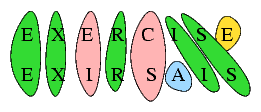
\includegraphics[scale=0.35]{images/edit2.png}
\end{center}
\item String Edit distance algorithm for spelling correction:
\begin{figure}[ht]
\begin{center}
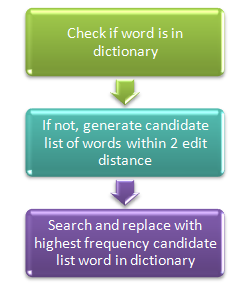
\includegraphics[scale=0.5]{images/editdistance.png}
\end{center}
\end{figure}
%Our edit distance algorithm corrects non-real word spelling errors by making at most 2 operations of insertion, deletion and substitution of letters in the word. The choice of 2 is governed by the trade off between algorithm runtime and quality of spelling correction. The spelling corrector has been designed as suggested by Peter Norvig http://norvig.com/spell-correct.html.

\item  The choice of 2 is governed by the trade off between algorithm
runtime and quality of spelling correction. 
%\item Precompiled dictionary is used to search for candidate list of words within edit distance 2 from the word to be corrected
%\item Word correction is done by replacement with the highest frequency word and lowest edit distance among the candidate list of words

\end{itemize}
\end{frame}

\subsection{Spelling Correction Evaluation}
\tableofcontents[currentsection,currentsubsection]

\begin{frame}
\frametitle{Spelling Correction Evaluation}

\begin{itemize}
 \justifying

\item
Required to measure the performance of spelling correction\\ \vspace{0.2in}
\item
Evaluation Parameters:
\end{itemize}
\begin{enumerate}
\item \alert{ Accuracy} : measures the percentage of actual errors that get corrected in the OCR text after spelling correction and defined as follows:
$$Accuracy=  \dfrac{TP+TN} {TP+ FP + TN + FN}$$


where, 

$TP$=Number of True Positives,

$TN$=Number of True Negatives,

 $FP$=Number of False Positives,

 $FN$=Number of False Negatives.



\item \alert{Time taken} to run Spelling Correction Algorithm
\end{enumerate}
\end{frame}


\begin{frame}
\frametitle{Spelling Correction Evaluation (SCE) Algorithm}
\begin{itemize}
 \justifying

\item Word by word correspondence between corrected and original dataset not possible because of Word Split and Join errors in OCR dataset
\item SCE algorithm performs word by word automatic evaluation on post spell corrected OCR dataset using an n-word grams approach
%\item Algorithm uses an n-word grams approach by considering a window of k words before and after each word in the original text for each word in the corrected text
%\item Each word in the corrected text is marked as a True Positive, True Negative, False Positive, False Negative based on whether the spelling had been corrected and if a match is found in the k words window of the original text
%The choice of N=2 is based on the Word Split and Join errors in the dataset. This value can be set appropriately by considering the maximum difference of lengths in each line of OCR and original text in the dataset.
\end{itemize}

\begin{columns}
\column{0.7\textwidth}
%\begin{figure} [!htb]
\centering
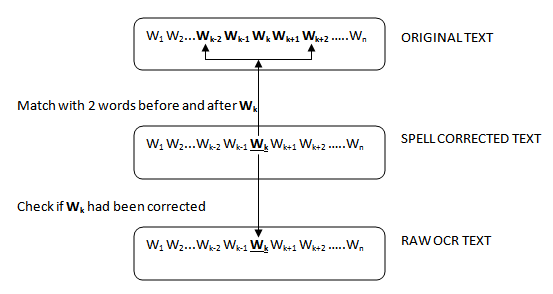
\includegraphics[scale=0.5]{images/ngram}
%\end{figure}

\column{0.3\textwidth}
%\begin{figure} 
\centering
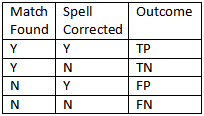
\includegraphics[scale=0.5]{images/ngram2}
%\caption{Schematic diagram for alignment of spell corrected article text with original article text for a word $W_{k}$}
%\end{figure}

\end{columns}
\begin{figure}
\caption{Schematic diagram for alignment of spell corrected article text with original article text for a word $W_{k}$}
\end{figure}
\end{frame}



\begin{frame}
\frametitle{Example}

\begin{block}{Line text from 3 versions of a news article:}
OcrLine= \textit{Irnniluttry iiownllllnu at tilchmond}\\

CorrectedLine= \textit{Irnniluttry iiownllllnu at Richmond}\\

OriginalLine= \textit{Grand jury now sitting at Richmond} 
\end{block}

\begin{table}[bt]
\begin{tabular}{|p{2.5cm}|p{4.5cm}|p{2cm}|} \hline
\textbf{Word in Corrected Line} & \textbf{Corresponding Word Window in Original Line}& \textbf{Result} \\ \hline
Irnniluttry & Grand jury now & FN \\ \hline
iiownllllnu & Grand jury now sitting & FN \\ \hline
at & now sitting at Richmond & TN \\ \hline
Richmond  &  sitting at Richmond & TP \\ \hline
\end{tabular}
\end{table}
\end{frame}

\begin{frame}
\frametitle{Spelling Correction Evaluation Results}
\begin{itemize}

 \justifying
\item
SCE algorithm tested on 50 spell corrected articles using 3 versions of each article: Original text, Raw OCR text and Spell Corrected text

\begin{block}{}
Accuracy :  $73.1 \%$\\
Time taken : 9 seconds on average per article
\end{block}


\item
We believe that the results are less accurate due to the presence of a large number of non-word, new line, word split and join errors in the OCR data which can not
be corrected by the edit distance spelling corrector used for this research.
\end{itemize}
\end{frame}



\section{Discussion}

\begin{frame}[allowframebreaks]
\frametitle{Discussion}
\begin{itemize}
 \justifying

\item
Spelling Correction accuracy can be improved by correcting other OCR errors like New Line and Word Split and Join errors
\item
 Choice of a dictionary for the edit distance algorithm affects the results of spelling correction 
\item
The choice of window size N=2 in SCE algorithm is based on the Word Split and Join errors in the dataset. This value can be set appropriately
by considering the maximum difference of lengths in each line of OCR and original text in the dataset.
\item
A limitation of the SCE algorithm is that it requires all 3 versions of a newspaper article (Original, Corrected and
OCR) to have the same number of lines as alignment of line texts is performed. In case of difference in the number of
lines of text due to some Word Split and Join errors, the word’s window needs to be extended so as to cover previous
and next line texts also for alignment.

\item
We compared our N-gram based SCE algorithm with the LCS (Longest Common Subsequence) algorithm
The LCS of corrected and original text gives a list of matching corrected words found in the original text.
\item
Following the similar evaluation procedure of calculating accuracy as in the N-word gram approach, it was found that
there is no statistically significant difference in accuracy when using either of the two algorithms.
\item
 We posit that LCS is a special case of the N-word gram algorithm when the window size N is set to the complete text in a line.
\end{itemize}
\end{frame}

\section{Conclusion and Future Work}
\begin{frame}
\frametitle{Conclusion and Future Work}
\begin{itemize}
 \justifying

\item
Proposed a novel approach and highlighted challenges for evaluating a spell correction algorithm on noisy OCR dataset through N-word grams alignment of the OCR, corrected and manually cleaned text.

\item
Preliminary results of application of our algorithm on an Edit distance based spell corrector evaluate its accuracy to be 73.1%.

\item
SCE algorithm can be used to compare among multiple spell correction algorithms and decide which one suits the dataset better and gives best accuracy

\item
In future, we plan to use other spelling correction algorithms like context dependent spelling correction to correct the OCR text and
measure the accuracy using our SCE algorithm


\end{itemize}
\end{frame}

\section{Acknowledgements}
\begin{frame}
\begin{block}{Acknowledgements}
This work was initially supported by the National Endowment of Humanities grant no. NEH HD-51153- 10. \\
The authors would like to thank Barbara Taranto and Ben Vershbow from the NYPL Labs for providing the article level newspaper data and Manoj Pooleery, Deepak Sankargouda and Megha Gupta for setting up the database used in this research.
\end{block}
\end{frame}

\begin{frame}

\begin{center}
\usebeamerfont*{frametitle} \usebeamercolor[fg]{frametitle}
\Huge Thank You.\\ \vspace{0.2in}
%Questions?
\end{center}
\begin{figure}[ht]
\begin{center}

\includegraphics[scale=0.5]{images/question.jpg}

\end{center}
\end{figure}

\end{frame}

\section*{References}
\begin{frame}

\frametitle{References}

\scriptsize{\bibliographystyle{acm}}

\bibliography{pptbib} %bibtex file name without .bib extension

\end{frame}


%EXTRA SLIDES


\begin{frame}
    \scalebox{0.65}{\begin{minipage}{1.53846\textwidth}

\begin{table}[h]
\centering
\caption{Different cases for word alignment in SCE algorithm}
\label{table2}

\begin{tabular}{|l|l|l|}
\hline
\backslashbox{Token index of CorrectedLine(i)}{Token index of OriginalLine}                                                   & Starting index (j)         & Ending index (j)         \\ \hline
Length{[}CorrectedLine{]} \textless4 or Length{[}OriginalLine{]}\textless4                                 & 0                          & Length{[}OriginalLine{]} \\ \hline
i=0                                                                                                        & 0                          & 3                        \\ \hline
i=1                                                                                                        & 0                          & 4                        \\ \hline
i=Length{[}CorrectedLine]-2 	&i-2			&Length{[}OriginalLine{]} \\ \hline
i=Length{[}CorrectedLine{]}-1	 & i-2                        & Length{[}OriginalLine{]} \\ \hline
i=Length{[}CorrectedLine{]}	 & i-2                        & Length{[}OriginalLine{]} \\ \hline
i=Length{[}CorrectedLine+1{]} & i-2                        & Length{[}OriginalLine{]} \\ \hline
i\textgreater=Length{[}CorrectedLine{]}+2                                                                  & Length{[}OriginalLine{]}-3 & Length{[}OriginalLine{]} \\ \hline
Any other value of i                                                                                            & i-2                        & i+3                      \\ \hline
\end{tabular}
\end{table}
\end{minipage}}
\end{frame}



\begin{frame}
    \scalebox{0.65}{\begin{minipage}{1.53846\textwidth}

\begin{algorithm}[H]
\caption{MatchWordGrams function of SCE Algorithm for measuring accuracy }
\begin{algorithmic}
\Function {MatchWordGrams}{OcrLine, CorrectedLine, OriginalLine, jstart, jend, i}
  
 \For{(int j=jstart; j$<$jend; j++)}
  {
    \If{ ((CorrectedLine[i].equals(OriginalLine[j]))\&\&(!(OcrLine[i].equals(CorrectedLine[i]))))}
     {
	  $tp=tp+1$\;
	  flag0=false\;
	 \Return $tp$\;
	  }
	\ElseIf{((CorrectedLine[i].equals(OriginalLine[j]))\&\&(OcrLine[i].equals(CorrectedLine[i])))}
	      {
		 $tn=tn+1$\;
		  flag1=false\;
		\Return $tn$\;
	      }
}

	 \If{(!(OcrLine[i].equals(CorrectedLine[i]))\&\&flag0==true)}
	 {
		    $fp=fp+1$\;
		   \Return $fp$\;
            }
	 
	 \ElseIf{((OcrLine[i].equals(CorrectedLine[i])) \&\& flag1==true)}
	 {
		    $fn=fn+1$\;
		   \Return $fn$\;
	 }
\EndFunction
\end{algorithmic}
\end{algorithm}%
\end{minipage}}
\end{frame}


\end{document}